%\RequirePackage[l2tabu, orthodox]{nag}

\documentclass{article}

\definecolor{bg}{rgb}{0.97,0.97,0.97}

% -- Bibliography
%\usepackage{csquotes}
%\usepackage{biblatex}
%\addbibresource{main.bib}

% -- Extra math options
\usepackage{mathtools}
\usepackage{siunitx} % Required for alignment
\sisetup{
  round-mode          = places, % Rounds numbers
  round-precision     = 2, % to 2 places
}

% -- Extra symbols
\usepackage{amssymb}
\usepackage{textcomp}
\usepackage{gensymb}
\usepackage{cancel}

% --  Image and float settings
\graphicspath{{graphics/}}
\usepackage{caption}
\usepackage{subcaption}
\usepackage{pdfpages}

% -- Graphs and diagrams
\usepackage{tikz}
\usepackage{pgfplots}
\usetikzlibrary{arrows.meta,positioning}
\pgfplotsset{compat=1.5, table/search path = {data}}

% -- Code listings
\usepackage{minted}
\setminted{linenos, bgcolor = bg, breaklines}
\setmintedinline{bgcolor = {}} 

% -- Extra table configs
\usepackage{booktabs}

\usepackage{siunitx} % Required for alignment
\sisetup{
  round-mode          = places, % Rounds numbers
  round-precision     = 2, % to 2 places
}
\definecolor{bg}{rgb}{0.95,0.95,0.95}
\setminted[c]{linenos, bgcolor = bg, breaklines}
\setmintedinline[c]{bgcolor = {}} 

\begin{document}

\begin{titlepage}


\includegraphics[viewport=9.5cm 11cm 0cm 0cm,scale=0.29]{IST_A_CMYK_POS}
	
\begin{center}
	\vspace{40mm} % --  Espaço em branco
	\rule{\linewidth}{0.5pt} \\
    \vspace{2mm}
	\Huge \textbf{Flight Management System and Dead-Reckoning Navigation} \\
	\rule{\linewidth}{2pt} \\
	\vspace{8mm} % -- Espaço em branco
	\Large Design of a Flight Management System and implementation of dead-reckoning navigation
	
	\vspace{\fill} % --  Espaço em branco variável
	
	\normalsize
	\begin{tabular}{r l}
		Pedro \textsc{Afonso} & \textbf{66277} \\
		João \textsc{Manito} & \textbf{73096} \\
		Daniel \textsc{de Schiffart} & \textbf{81479}
	\end{tabular}
	
	\vspace{10mm} % --  Espaço em branco
	\Large Instituto Superior Técnico \\
	Integrated Master's Degree in Aerospace Engineering \\
	\vspace{1mm}
	\large Integrated Avionic Systems
	
	\vspace{10mm} % --  Espaço em branco
	\Large $2018/2019$
\end{center}

\end{titlepage}

{\hypersetup{linkcolor = black} \tableofcontents}

\begin{abstract}
	For the first laboratory of the course of Integrated Avionic Systems the objective was to design a simple version of a \emph{Flight Management System} and use it to simulate a navigation across a series of pre-defined waypoints across a sphere-shaped earth. Further on, the development focused on the study of dead-reckoning navigation, its implementation within the Flight Management System and the comparison of a simulation with this feature against the original simulation. The final part of the laboratory shifted the focus to possible errors within the acquisition of flight velocity within the flight and ways to reduce these errors to obtain more accurate navigation. The entire work was to be implemented in C code and use a basic interface of both terminal and text-files for input and output of information.
\end{abstract}

\part{Route Distance}

The first part of this laboratory project was to develop the basic functions to allow for basic simulated navigation. With the final objective of this part being to determine the total distance of a path comprised of a series of waypoints, the work was split into different components to allow for streamlined development.

\section{Definition of Coordinates on a Spherical Earth}

On a spherical Earth, the coordinates are given in latitude and longitude in relation to a reference equator and meridian, while altitude is given as the difference between a certain point's distance to the center of the Earth and the spherical Earth's radius. The value of the Earth's radius was defined as being $6378000$ meters.

With this environmental information, the obvious approach for saving the data of waypoints and positions in the code would be with a definition of a C structure. Our code implements a \mintinline{c}{struct} with the \mintinline{c}{typedef} name of \mintinline{c}{Coord}.

\section{Distance Determination} \label{sec:dist_det}

To determine the distance between two coordinates on a spherical earth, the first objective is to determine the distance of the shortest great-circle path. As we assume that the altitude (and therefore the radius) of the path is constant for each segment of the flight, this can be done using the radial distance between the two points and multiplying it by the radius of the path. Using $\phi$ as latitude and $\lambda$ as latitude, the radial distance $\theta$ between points $1$ and $2$ is given by equation \ref{eq:raddist}.
\begin{gather} \label{eq:raddist}
    \theta = \cos^{-1}{\left(\cos\phi_2\cos\left(\lambda_1 - \lambda_2\right)\cos\phi_1 + \sin\phi_2\sin\phi_1\right)}
\end{gather}
Defining the Earth radius as $R$ and the height of any coordinate as $h$, we can finally obtain the distance of the great-circle path between two coordinates as $d$, which is given by equation \ref{eq:raddist_m}.
\begin{gather} \label{eq:raddist_m}
    d = \theta \times (R + h_1)
\end{gather}
These equations have been implemented as C functions in the file \texttt{lab1.c}.

Applying this to a sequencial set of waypoints is a matter of iteration and cumulative sums to determine the total distance. However, an issue is raised when the altitude is not constant between points, as we consider the altitude constant between any two waypoints using the value of the first point of any segment. This will lead to some error in the measurement of altitudes, as sudden jumps of altitude will distort the distance travelled from reality by a little bit. The focus of this discussion is illustrated by figure \ref{tikz:consth_error} in two dimensions.
\begin{figure}[ht]
    \centering
    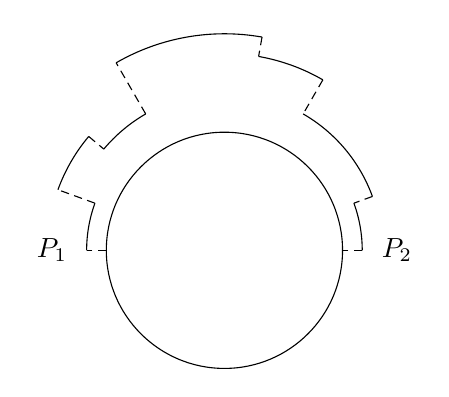
\begin{tikzpicture}[x = 0.5cm, y = 0.5cm, climb/.style={densely dashed}]
        \node (main) at (0,0) {};
        \draw  (main) ellipse (3 and 3);
        \draw (-3.5,0) node (v1) [label = {180:$P_1$}] {} arc (180:160:3.5);
        \draw (-4.2286,1.5391) node (v3) {} arc (159.9998:140:4.5);
        \draw (-3.0642,2.5712) arc (139.9997:120:4);
        \draw (-2.75,4.7631) arc (120.0002:80:5.5);
        \draw (0.8682,4.924) arc (80.0004:60:5);
        \draw (2,3.4641) arc (60:20:4);
        \node (v2) at (-3,0) {};
        \draw (3.2889,1.1971) arc (20.0006:0:3.5);
        \node (v4) at (3.5,0) [label = {0:$P_2$}] {};
        \draw [climb] (180:3) -- (180:3.5);
        \draw [climb] (160:3.5) -- (160:4.5);
        \draw [climb] (140:4.5) -- (140:4);
        \draw [climb] (120:4) -- (120:5.5);
        \draw [climb] (80:5.5) -- (80:5);
        \draw [climb] (60:5) -- (60:4);
        \draw [climb] (20:4) -- (20:3.5);
        \draw [climb] (0:3.5) -- (0:3);
    \end{tikzpicture}
    \caption{Simulation of the implemented distance calculation algorithm in 2D. Notice the separation of segments, the constant altitude in each of them and the unrealistic jumps of altitude between each of them.}
    \label{tikz:consth_error}
\end{figure}

\part{Dead-Reckoning Navigation}

The second part of this laboratory project developed on the work of the previous part to simulate a full flight from start to finish and to observe the effect of extra modifications and fixes on the accuracy of the final simulation. For that purpose, a flight plan comprised of waypoints was devised and a speed condition was applied to each segment.

\section{Flight Path Definition} \label{sec:fpath}

For a simulation to occur, a flight plan was necessary. According to the assignment, the flight plan was comprised of twelve cities, with the final waypoint being equal to the first waypoint. A value for the true airspeed was also selected for each segment, and stored in the waypoint that preceeded it. With this information, a set of coordinates was selected for each city using the city's airport as a reference. The list of waypoints can be found in table \ref{tab:waypoints}.
\begin{table}[ht]
    \centering
    \begin{tabular}{c c c c c}
        \hline
        City            & Latitude              & Longitude             & Altitude ($ft$) & TAS (\si{\meter\per\second})  \\
        \hline
        Lisbon          & $38.7812995911$       & $-9.13591957092$      & 374   & 200     \\
        Paris           & $49.0127983093$       & $2.54999995232$       & 392   & 300     \\
        Moscow          & $55.40879821777344$   & $37.90629959106445$   & 588   & 200     \\
        Oslo            & $60.193901062012$     & $11.100399971008$     & 681   & 500     \\
        Rome            & $41.8002778$          & $12.2388889$          & 13    & 250     \\
        Madrid          & $40.471926$           & $-3.56264$            & 1998  & 300     \\
        Funchal         & $32.697898864746$     & $-16.774499893188$    & 192   & 400     \\
        Ponta Delgada   & $37.7411994934$       & $-25.6979007721$      & 259   & 700     \\
        New York        & $40.63980103$         & $-73.77890015$        & 13    & 500     \\
        Halifax         & $44.8807983398$       & $-63.5085983276$      & 477   & 200     \\
        London          & $51.4706$             & $-0.461941$           & 83    & 100     \\
        Lisbon          & $38.7812995911$       & $-9.13591957092$      & 374   & 250     \\
        \hline
    \end{tabular}
    \caption{Waypoints of the flight path used in this part of the laboratory project. Latitude and longitude are represented in decimal degrees, altitude is in feet and true airspeed is in meters per second.}
    \label{tab:waypoints}
\end{table}

\subsection{Waypoint input}

The input of these waypoints was done using a comma-separated value text file (henceforth referred to as \texttt{csv}). The data found in table \ref{tab:waypoints} was left as-is when introduced into the file, using commas to separate each column in a line, removing all whitespace utilized (except in the header line).

For this information, we created a separate structure from the \texttt{Coord} structure used previously to allow for the storage of more information. We called this structure \texttt{Waypoint}, which was defined as seen in file \texttt{waypoints.h}.

The file is read by calling the function \mintinline{c}{read_file}, and the waypoints are returned in a \mintinline{c}{Waypoint} array whose pointer was provided as an argument to the function. We decided to use the function \mintinline{c}{fgets} in loop to get all the lines with the waypoints written. Inside the loop, longitude, latitude, altitude and true airspeed values are stored in a \texttt{Waypoint} structure. The function \mintinline{c}{csv_waypoint_parse(char line[])} receives a string containing a line of the waypoint file and returns the obtained values inside a \texttt{Waypoint} structure. The separation of each value inside the line string was done using the \texttt{strtok}, using the expected comma token.

\subsection{Theoretical distance for the flight plan}

To allow for the waypoint data stored in the received array to be used with the remaining functions, a \texttt{Coord} structure had to be extracted from every used waypoint. The function \mintinline{c}{waypoint_to_coord()} covers that functionality, receiving the stored data and making it usable with the necessary functions, by converting its latitude and longitude to radian format and converting the altitude to the corresponding value in SI units (in this case, meters).

The function \mintinline{c}{coord_dist()} receives the two waypoints and compute its distance. The formula is equation \ref{eq:raddist_m} and was explained in section \ref{sec:dist_det}.

\section{Flight Simulation} \label{sec:flightsim_basic}

Using the waypoints obtained in section \ref{sec:fpath}, we can now start running a virtual simulation of a flight that runs a flight path comprised of the referred waypoints. This section covers the basic procedure of a simulation using constant $V_{TAS}$ between each waypoint, for which the value is obtained from the waypoint file already referenced. The simulation herein described will therefore act as a frame of reference for further simulations.

The $V_{TAS}$ used in a segment of the flight path corresponds to the value obtained from the segment's starting waypoint.

\subsection{Velocity and distance}

For the present work, we used two separate methods for computing the position. For the first lab question, we used constant $V_{TAS}$ for each leg of the flight. The trajectory between the two waypoints was divided by segments that we called subpoints. The distance between two subpoints is defined by the true aispeed and time span relation. If we define $D$ as the distance between two consecutive waypoints and $d$ as the distance covered in each simulation step, with each step being a fixed $\Delta t$ of time, at speed $V_{TAS}$, we can use the relations to find the number of subpoints $n$ in a segment.
\begin{gather*}
    d = V_{TAS} \times \Delta t \Rightarrow n = \frac{D}{d}
\end{gather*}

On the other hand, the $\theta_{path}$ is given by
\begin{gather*}
    \theta_{path} = arcsen\left(\frac{\frac{dh}{dt}}{v_{TAS}}\right)
\end{gather*}
where the altitude rate $dh/dt$ is given by
\begin{gather*}
    \frac{dh}{dt}=-\alpha h(t) - \alpha h_r(t)
\end{gather*}
at any given time, where $h(t)$ is the current altitude and $h_r(t)$ the current target altitude.

\subsection{True heading} \label{sec:theading}

The true heading is obtained by a function \mintinline{c}{depheading(position_current, waypoint_next_coor)} which receives the current position, in a specific subpoint and the following waypoint. This is the formula to get $\psi_T$ from the coordinates of two different points: 
\begin{gather*}
    \psi_T = \tan^{-1}\left(\frac{-\cos\phi_2\sin(\lambda_1 - \lambda_2)}{-\cos\phi_2\cos(\lambda_1 - \lambda_2)\sin\phi_1 + \sin\phi_2\cos\phi_1}\right)
\end{gather*} 

\subsection{Refreshing the segment position}

For each time $t$, there is a true heading. So a loop was implemented with \mintinline{c}{coord_fromdist}. This new function gives us the next subpoint exact position, with the new coordinates. The input is the current position, the distance travelled, the heading and the climb. The two coordinates are given by the following formulas:
\begin{align*}
    \phi_2 &= \sin^{-1}\left(sin(\phi_1)\cos\left(\frac{d}{R}\right) + \cos\phi_1\sin\left(\frac{d}{R}\right)\cos\psi\right) \\
    \lambda_2 &= \lambda_1 + \tan^{-1}\left(\frac{\sin\psi\sin\left(\frac{d}{R}\right)\cos\phi_1}{\cos\left(\frac{d}{R}\right) - \sin\phi_1\sin\phi_2}\right)
\end{align*}  

To end the loop, the log file is updated with the new data. All the process is repeated again for each trajectory segment until arrive to the next waypoint.

The heading of the aircraft throughout the flight path can be seen in figure \ref{fig:heading}.
\begin{figure}[ht]
    \centering
    \begin{tikzpicture}
    	\begin{axis}[   width = 0.9\linewidth, height = 7cm,
    	                xlabel = {Time (\si{\second})},
    	                ylabel = {Heading (\si{\radian})},
    	                grid = both,]
    		\addplot [red] table [col sep = comma, x index = 0, y index = 1, mark = none] {p1_heading.csv};
    	\end{axis}
    \end{tikzpicture}
    \caption{Aircraft heading through the flight path.}
    \label{fig:heading}
\end{figure}

\section{Modified Simulations}

As part of the assignment, the simulation described in section \ref{sec:flightsim_basic} and the conditions of said simulation were to be modified and the results observed and compared.

\subsection{Iteration velocity and distance}

Since a time-dependent simulation was required for the remaining simulations, a Flat-Earth Approximation was used. By using the coordinates of the first point as reference, and for short distances, we can define a local ENU referential. We can compute the $V_{TAS}$ components in that referential
\begin{align*}
    V_{East}(t) &= V_{TAS}(t)\cos\left(\theta_{path}(t)\right)\sin\left(\phi_T(t)\right) \\
    V_{North}(t) &= V_{TAS}(t)\cos\left(\theta_{path}(t)\right)\cos\left(\phi_T(t)\right) \\
    V_{Up}(t) &= V_{TAS}(t)\sin\left(\theta_{path}(t)\right)
\end{align*}
and then obtain the position change in ENU components as
\begin{align*}
    \Delta E &= V_{East} \times \Delta t \\
    \Delta N &= V_{North} \times \Delta t \\
    \Delta U &= V_{Up} \times \Delta t
\end{align*}
Using the radius of the sphere where the airplane is located, 
\begin{align*}
	R = R_{Earth} + h
\end{align*}
we can convert the changes in ENU coordinates to changes in the ECEF referential
\begin{gather*}
    \Delta \phi = \frac{\Delta N}{R} \\
    \Delta \lambda = \frac{\Delta E}{R \times \cos\phi_1}
\end{gather*}
The new coordinates are obtained by adding the computed changes to the initial point
\begin{align*}
    \phi_2 &= \phi_1 + \Delta \phi \\
    \lambda_2 &= \lambda_1 + \Delta \lambda \\
    h_2 &= h_1 + \Delta h
\end{align*}

Since this approximation depends on the simulation's temporal resolution, the smaller the time increment the more realistic will be the result.

\subsection{Non-ideal Sensor}

The first test scenario was to include an error in the measured airspeed, which to this point was considered to be constant throughout any segment between waypoints. This sensor would cause a modification to the detected airspeed, which will inevitably cause differences in the final result.

The error measurements caused by the sensor with respect to time $t$, with $T=\SI{20}{\minute}$, are
\begin{gather*}
    V_m(t) = V_{TAS}\left(1+0.01 \times sen\left(\frac{2\pi t}{T}\right)\right)
\end{gather*}

Inside the loop, for each subpoint, we store now two different $\theta_{path}$ with the same function \mintinline{c}{thetapath}. The first one receives as input the True Air Speed and the position current true. However the second one, that we called \mintinline{c}{theta_sensor}, receives as input the position current relative to the sensor and the speed given by the sensor with a natural error, \mintinline{c}{Vm}.
\par So, there are also two different positions, named \mintinline{c}{position_current_true} and \mintinline{c}{position_current_sensor} which are calculated with the same heading. Using the function \mintinline{c}{update_position} refresh both the measured(virtual) and the real positions during the simulation. The first one receives \mintinline{c}{theta_true}, its previous position and True Air Speed, as the second one receives the speed read by the sensor, \mintinline{c}{theta_sensor} and its previous position. 
\par Each $t$ means 1 minute, the unit chosen for the simulation time scale. After running the simulation, the difference between the two subpoints obtained are printed in the logfile.
\par After reading the log file, it's clear the error is increased after each waypoint as we expected. By the other side, between two subpoints sometimes the error in the current subpoint is smaller than its previous subpoint. In a large number of subpoints, a major error can be observed when we compare the first one with the last one. The error is being accumulated after crossing each waypoint.

\subsection{Feedback Speed Controller} \label{sec:fsc}

To mitigate the noise generated by the airspeed sensor, a feedback speed controller was devised. The controller takes the desired (reference) airspeed, $V_{ref}$, and the current airspeed, computes the error and returns a control signal to the actuators. The implemented controller is a Proportional - Integrative (PI) controller. This type of controller was selected because it provides a good convergence speed as well as removing the static error. The controller (in its time-domain form) is defined by
\begin{gather*}
    u(t)=K_pe(t)+K_i\int_0^t e(t)
\end{gather*}
Where $u(t)$ is the control signal, $e(t)$ is the airspeed error relative to $V_{ref}$ and $K_i$ and $K_p$ are, respectively, the integral and proportional control constants . This control signal is then fed to the actuators. For the present simulation, the simulated actuator is a simple delay of one simulation time step:
\begin{gather*}
    V_{TAS}(t)=u(t-1)
\end{gather*}

For this simulation, we chose $K_i$ and $K_p$ in a relatively loose way, since the determination of precise values for these constants was regarded as outside the main scope of this lab. We then obtained $K_i=0.001$ and $K_p=0.5$.

\subsection{Results Analysis}
The errors are decreased when a controller is used. There is an improvement on the reference following and the Velocity measured by the sensor. it was explained in subsection \ref{sec:fsc}. The Proportional Gain improves the following reference and the Integrative Gain makes the static error 0.

From the analysis of the results, we can clearly see that the usage of the Dead-Reckoning method significantly decreases the positioning errors, due to its capability to reset the position error when a waypoint is reached. However, when using just a simple speed controller there were unexpected results. While in some cases the error using the controller is smaller than the error obtained using the noisy $V_{TAS}$ signal as expected, in other cases the error was bigger. This is almost certainly due to a incorrectly designed controller, where the parameters aren't good enough for this problem. There is also a possibility that the added actuator delay is also responsible for some of the error, since the delay is a full simulation time step, in this case 1 minute, which makes the response of the system lag considerably to a control signal.
\\
There is also an interesting segment of the simulation, the Oslo-Rome leg, where the Dead Reckoning error is larger than the error given by both the noisy airspeed signal and the controller. Most likely this is also a consequence of the bad controller design.\\
\\
Globally, we can consider the simulation successful, but requiring additional testing and calibration of the controller, as well as a smaller simulation step to avoid the high lag between control signal and actuator.

\\
\begin{table}[h!]
  \begin{center}
    \caption{Position error at the waypoints}
    \label{tab:table1}
    \begin{tabular}{S|S|S|S} % <-- Alignments: 1st column left, 2nd middle and 3rd right, with vertical lines in between
      \textbf{Waypoint} & \textbf{Noise} & \textbf{Controller} & \textbf{DR + Controller}\\
      \hline
      1 & 0.0 & 0.0 & 0.0\\
      2 & 210.312050 & 300.096244 & 298.006947\\
      3 & 511.685851 & 771.749607 & 144.360239\\
      4 & 607.941173 & 769.452356 & 163.469602\\
      5 & 1294.716001 & 1295.054737 & 2009.739342\\
      6 & 1483.407847 & 1436.921079 & 764.300514\\
      7 & 1440.604287 & 1556.405695 & 134.720407\\
      8 & 1284.097342 & 1383.566351 & 470.251469\\
      9 & 466.548364 & 1383.566351 & 1212.794061\\
      10 & 1060.093213 & 816.023553 & 211.371189\\
      11 & 1503.284270 & 1585.098214 & 61.817500 \\
      12 & 1729.362248 & 1786.824637 & 33.652273 \\
    \end{tabular}
  \end{center}
\end{table}

\begin{figure}[ht]
    \centering
    \begin{tikzpicture}
    	\begin{axis}[   width = \linewidth, height = 7cm,
    	                xlabel = {Time (\si{\second})},
    	                ylabel = {Error (\si{\meter})},
    	                grid = both,legend pos = north east]
    		\addplot table [col sep = comma, x index = 0, y index = 1, mark = none] {p2_error.csv};
    		\addplot table [col sep = comma, x index = 0, y index = 1, mark = none] {p3_error.csv};
    		\addplot table [col sep = comma, x index = 0, y index = 1, mark = none] {p4_error.csv};
    		\legend{A, B, C}
    	\end{axis}
    \end{tikzpicture}
    \caption{Subpoints distances error between the real position using TAS and the measured position using the velocity sensor -- blue. Subpoints distances error between the real position using TAS and the measured position using the controller with the velocity sensor -- red. Subpoints distances error between the real position using TAS and the measured position using the controller and sensor with correction of true position in the waypoints -- brown.}
    \label{fig:error_all}
\end{figure}

\end{document}
